%%%%%%%%%%%%%%%%%%%%%%%%%%%%%%%%%%%%%%%%%%%%%%%%%%%%%%%%%%%%%%%%
%                      REMESHING
%%%%%%%%%%%%%%%%%%%%%%%%%%%%%%%%%%%%%%%%%%%%%%%%%%%%%%%%%%%%%%%%
\chapter[Remeshing]{Remeshing} \label{appendix:remeshing}

In Chapter~\ref{chap:cutting}, topological changes are applied on the visual model which is a triangular mesh. As the mesh is only used for visualization. Simulation robustness will not be determined by its elements' quality. Therefore we used an extremely simple remeshing algorithm. The input are the mesh and a polyline that represents the cut. We start by remeshing along the polyline so that the mesh  conforms with it. Then we duplicate the mesh vertices along this polyline to create the crack. The whole procedure is summarized in algorithm \ref{alg:remeshing} and illustrated in Figure \ref{fig:remeshing}. The remeshing part uses vertex insertion and edge split operations (see Figure \ref{fig:operations}). The splitting part only uses vertex split operation (see Figure \ref{fig:vertexSplitting}).

\begin{algorithm}[hp]
\caption[Frame-based cutting: Remeshing algorithm]{\label{alg:remeshing}Remeshing Algorithm}
\begin{algorithmic}[1]
\Procedure{Cut$\_$Along$\_$Segment}{Segment $S$, mesh $M$}
\State \textsc{Insert$\_$Segment}($S$, $M$)
\State $\tilde{P} \gets$ edges corresponding to $S$
\State \textsc{Split$\_$Along$\_$Polyline}($\tilde{P}$,$M$)
\EndProcedure
\State
\Procedure{Insert$\_$Segment}{Segment $S$, Mesh $M$}
\State $\tilde{S} \gets$ subdivide $S$ at intersection with $M$ edges
\For{each point $i$ of $\tilde{S}$}
\State $E \gets$ closest edge to $i$
\State $V \gets$ closest vertex to $i$
\State $F \gets$ closest triangle to $i$
\If{distance($E$,$i$)$<\epsilon_{edge}$}
\State Split $E$ at $i$
\ElsIf{distance($V$,$i$)$<\epsilon_{vertex}$}
\State Snap $i$ to $V$
\Else
\State Split $F$ at $i$
\EndIf
\EndFor
\EndProcedure
\State
\Procedure{Split$\_$Along$\_$Polyline}{Polyline $P$, Mesh $M$}
\For{each vertex $V$ of $P$}
\State Split triangles around $V$ according to $P$
\EndFor
\EndProcedure
\end{algorithmic}
\end{algorithm}

\clearpage 

\begin{figure}[p]
\centering
\begin{subfigure}[c]{0.3\linewidth}
\centering
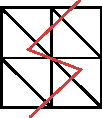
\includegraphics[height=3.5cm]{images/cutting-mig2015/remeshing_1.pdf}
\caption{\label{fig:remeshing1}}
\end{subfigure}
\hfill
\begin{subfigure}[c]{0.3\linewidth}
\centering
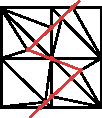
\includegraphics[height=3.5cm]{images/cutting-mig2015/remeshing_2.pdf}
\caption{\label{fig:remeshing2}}
\end{subfigure}
\hfill
\begin{subfigure}[c]{0.3\linewidth}
\centering
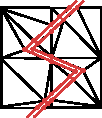
\includegraphics[height=3.5cm]{images/cutting-mig2015/remeshing_3.pdf}
\caption{\label{fig:remeshing3}}
\end{subfigure}
\caption[Frame-based cutting: Remeshing algorithm]{\label{fig:remeshing} Illustration of our remeshing algorithm. (a) For remeshing, we start from an input mesh and a polyline that represents the cut. (b) First we re-mesh along the polyline so that the mesh is conform with the cut. (c) Then we split the mesh vertices along the polyline.}
\end{figure}

\begin{figure}[p]
\centering
\begin{subfigure}[c]{0.3\linewidth}
\centering

\includegraphics[height=3cm]{images/cutting-mig2015/basic_mesh.pdf}
\caption{\label{fig:basicMesh}}
\end{subfigure}
\hfill
\begin{subfigure}[c]{0.3\linewidth}
\centering

\includegraphics[height=3cm]{images/cutting-mig2015/edge_split.pdf}
\caption{\label{fig:edgeSplitting}}
\end{subfigure}
\hfill
\begin{subfigure}[c]{0.3\linewidth}
\centering
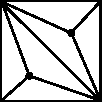
\includegraphics[height=3cm]{images/cutting-mig2015/vertex_insertion.pdf}
\caption{\label{fig:vertexInsertion}}
\end{subfigure}
\caption[Frame-based cutting: Edge splitting and vertex insertion]{\label{fig:operations} Illustrations for edge splitting and vertex insertions. (a) The input mesh. (b) After edge splitting. (c) After vertex insertions.}
\end{figure}

\begin{figure}[p]
\centering
\begin{subfigure}[c]{0.3\linewidth}
\centering
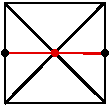
\includegraphics[height=3cm]{images/cutting-mig2015/vertex_splitting_1.pdf}
\caption{\label{fig:vertexSplitting1}}
\end{subfigure}
\begin{subfigure}[c]{0.3\linewidth}
\centering

\includegraphics[height=3cm]{images/cutting-mig2015/vertex_splitting_2.pdf}
\caption{\label{fig:vertexSplitting2}}
\end{subfigure}
\begin{subfigure}[c]{0.3\linewidth}
\centering

\includegraphics[height=3cm]{images/cutting-mig2015/vertex_splitting_3.pdf}
\caption{\label{fig:vertexSplitting3}}
\end{subfigure}
\caption[Frame-based cutting: Vertex splitting]{\label{fig:vertexSplitting} Illustrations for the vertex splitting operation. (a) A mesh which is conform with the polyline (in red). (b) We start by assigning each triangle around the vertex to split to one side of the polyline. (c) We duplicate the vertex and modify each of the triangles accordingly to its side.}
\end{figure}
